\section{Results: the ablation}\label{sec:ablation}

\subsection{The trained CNNs as identifiers}

The CNNs trained here are weak identifiers: \N{cos_clean_lo} to \N{cos_clean_hi}\% clean rank-1 for the four CosFace configurations, against \N{r1_arc_s00}\% for ArcFace and \N{r1_sf_s00}\% for SFace. Each is a \N{params_m}-million-parameter network trained from scratch on \N{n_train_images} crops of \N{n_train_identities} identities, while the pretrained models were trained on far larger face datasets. The comparison gives scale only; the study is about the differences between the trained configurations. Their CosFace loss was \N{cos_ep1_lo} to \N{cos_ep1_hi} in the first epoch and \N{cos_last_noaug_lo} to \N{cos_last_noaug_hi} (without augmentation) or \N{cos_last_aug_lo} to \N{cos_last_aug_hi} (with it) in epoch \N{epochs}.

Without augmentation, the CNNs fall fast on centered squares, from \N{r1_nn_s00}\% clean to \N{r1_nn_s10}\% at 10\% (``CNN, neither'') and from \N{r1_at_s00} to \N{r1_at_s10}\% (``CNN, attention''). With augmentation, they start lower and fall slowly: ``CNN, both'' identifies \N{r1_both_s00}\% clean, \N{r1_both_s20}\% at 20\%, and \N{r1_both_s50}\% at 50\% (Fig.~\ref{fig:squares}b).

\subsection{The three primary contrasts}

All three primary contrasts pass the decision rule of Section~\ref{sec:metrics} (Table~\ref{tab:primary} and Fig.~\ref{fig:contrasts}a). No bootstrap resample, with seeds drawn separately for each configuration, crossed zero for any of them, so each has $p<\N{P1_p}$ and Holm $p<\N{P1_holm}$, and each keeps its sign in every one of the \N{combos} one-seed-per-configuration combinations. With \N{n_seeds} seeds per configuration, though, the seed half of each resample can only redraw those \N{n_seeds} values. With seeds as the unit, P1 and P2 clear 0.05 in both of the following unadjusted $t$ analyses, and P3 clears it only in the first: a Welch-type $t$ on per-seed means, treating the configurations as independent, gives $p=\N{P3_seed_p}$ ($t=\N{P3_seed_t}$, \N{P3_seed_df}~df), while a $t$ on its \N{n_seeds} matched-seed values (each configuration's seed $s$ starts from the same seed) gives $p=\N{P3_pair_p}$ ($t=\N{P3_pair_t}$, \N{P3_pair_df}~df). P3 meets the bootstrap rule and is positive for every seed and seed combination, but with \N{n_seeds} seeds, its significance depends on the test.

\begin{table}[t]
\caption{The three primary contrasts (P1: augmentation on the trained-on squares; P2: augmentation on unseen occluders; P3: attention on the \N{n_p3} occluded conditions of P1 and P2): main effects on identity rank-1, in points, with 95\% and 98.3\% (Bonferroni over three) bootstrap intervals and the range over all \N{combos} one-seed-per-configuration combinations. Each has bootstrap $p<\N{P1_p}$ and Holm $p<\N{P1_holm}$; with seeds as the unit, P3 has $p=\N{P3_seed_p}$ or \N{P3_pair_p} (see the text).}
\label{tab:primary}
\centering\small
\setlength{\tabcolsep}{3pt}
% Generated by make_numbers.py. Do not edit.
\begin{tabular}{@{}lrrrr@{}}
\toprule
& Est. & 95\% interval & 98.3\% interval & Seed combos \\
\midrule
P1 & +12.1 & [+10.9, +13.4] & [+10.6, +13.7] & +11.4 to +12.7 \\
P2 & +5.2 & [+4.5, +6.0] & [+4.4, +6.2] & +4.5 to +5.8 \\
P3 & +1.0 & [+0.5, +1.5] & [+0.4, +1.6] & +0.5 to +1.7 \\
\bottomrule
\end{tabular}

\end{table}

\begin{figure*}[t]
\centering
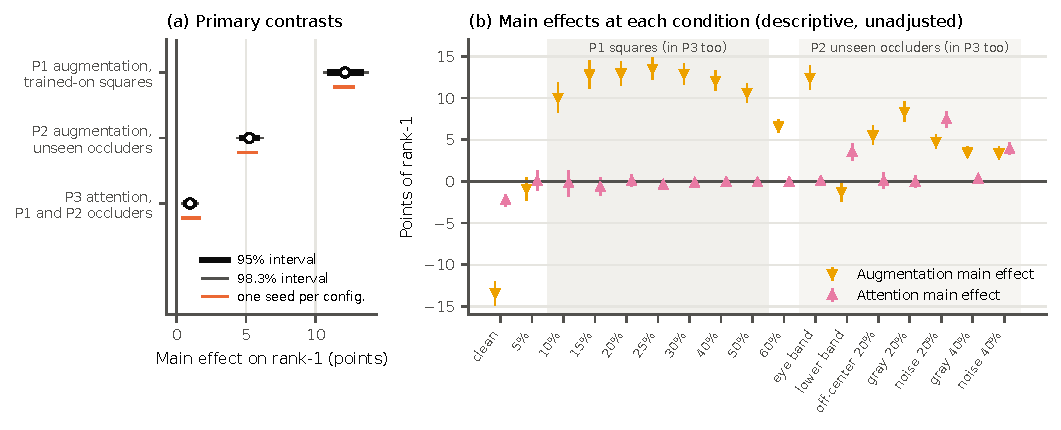
\includegraphics[width=\textwidth]{figures/fig_contrasts.pdf}
\caption{(a) The three primary contrasts: estimate (circle), 95\% interval (thick), 98.3\% interval (thin), and the range over the \N{combos} one-seed-per-configuration combinations (below). (b) The augmentation and attention main effects at each identity condition, with 95\% intervals; these are the terms P1 to P3 average over, shown for description only (unadjusted). Shading marks the conditions in P1 and in P2; P3 averages the attention terms over both.}
\label{fig:contrasts}
\end{figure*}

\subsection{Occlusion augmentation: a trade-off}

Augmentation's main effect is \N{P1} points [\N{P1_lo}, \N{P1_hi}] on the centered squares it trains with (P1) and \N{P2} [\N{P2_lo}, \N{P2_hi}] on the occluders it never saw (P2). It costs \N{aug_s00_abs} points [\N{aug_s00_hi_abs}, \N{aug_s00_lo_abs}] on clean faces. At a 5\% square, its effect is \N{aug_s05} [\N{aug_s05_lo}, \N{aug_s05_hi}], no detectable difference (Fig.~\ref{fig:contrasts}b). Transfer to the unseen occluders is uneven: \N{aug_eye} on the eye band, \N{aug_gray20} on a 20\% gray square, \N{aug_off20} on the off-center square, \N{aug_gray40} and \N{aug_noise40} at 40\% gray and noise, \N{aug_noise20} at 20\% noise, and \N{aug_low} [\N{aug_low_lo}, \N{aug_low_hi}] on the lower band. P2 supports transfer on average, not to every occluder. At the 60\% square, beyond the trained range, the effect is \N{aug_s60}.

The average combines two networks that behave differently. ``CNN, augmentation'' (no attention) has rank-1 at or below chance on both noise fills (\N{r1_au_noise20}\% and \N{r1_au_noise40}\%; \N{seed_au_noise20_min} to \N{seed_au_noise20_max}\% per seed at 20\%), so augmentation without attention changes rank-1 under 20\% noise by \N{sc_augN_noise20} points [\N{sc_augN_noise20_lo}, \N{sc_augN_noise20_hi}], while with attention, it adds \N{sc_augA_noise20}. Across seeds, though, the right identity's mean rank is \N{mrank_au_noise20_min} to \N{mrank_au_noise20_max} of \N{n_gallery} at 20\% noise and \N{mrank_au_noise40_min} to \N{mrank_au_noise40_max} at 40\%, ahead of guessing (about half the gallery). On the lower band, the pattern reverses: augmentation with attention changes rank-1 by \N{sc_augA_low} points [\N{sc_augA_low_lo}, \N{sc_augA_low_hi}], and without attention by \N{sc_augN_low}. These per-condition contrasts are descriptive: \N{sc_excl_n} of the \N{sc_n} simple contrasts on the identity protocol have a 95\% interval that excludes zero, unadjusted (\N{sc_cos_excl_n} of the \N{sc_cos_n} that leave out the \N{sc_tri_n} comparisons with the failed triplet runs), and about \N{sc_chance_n} would by chance alone if no contrast had an effect.

\subsection{Attention: noise fills and the lower band}

Attention's main effect over the \N{n_p3} occluded conditions of P1 and P2 (P3) is \N{P3} point [\N{P3_lo}, \N{P3_hi}]. Only \N{att_excl_n} of its \N{n_p3} terms have intervals that exclude zero, all positive: 20\% noise (\N{att_noise20}), 40\% noise (\N{att_noise40}), and the lower band (\N{att_low}). On the \N{n_trained_squares} trained-on squares, the terms run from \N{att_trained_min} to \N{att_trained_max} points, none with an interval excluding zero; with \N{n_seeds} seeds, that is no effect detected at this scale, not evidence of no effect. On clean faces, attention costs \N{att_s00_abs} points [\N{att_s00_hi_abs}, \N{att_s00_lo_abs}].

The noise-fill effect is concentrated in the augmented networks. With augmentation, the network without attention identifies \N{r1_au_noise20}\% and \N{r1_au_noise40}\% under 20\% and 40\% noise fills, and the one with attention \N{r1_both_noise20}\% and \N{r1_both_noise40}\% (a difference of \N{sc_attA_noise20} points [\N{sc_attA_noise20_lo}, \N{sc_attA_noise20_hi}] at 20\%). Without augmentation, attention adds \N{sc_attN_noise20} points at 20\% noise and \N{sc_attN_low} [\N{sc_attN_low_lo}, \N{sc_attN_low_hi}] on the lower band. In this setup, then, adding the attention layer took the augmented network's rank-1 from chance or below to \N{r1_both_noise20}\% and \N{r1_both_noise40}\% under noise fills it never saw in training, and did not help on the black squares it trained against. There, adding attention to the augmented network changed rank-1 by \N{sc_attA_s10} to \N{sc_attA_s25} points at the 10 to 25\% squares (descriptive, with unadjusted intervals that exclude zero); the main-effect terms average these with the changes without augmentation, \N{sc_attN_s15} to \N{sc_attN_s10} points on the same squares. Why the augmented network without attention fails on noise was not tested.

\subsection{Where the attention weight goes}

Table~\ref{tab:attention} gives the mean attention weight inside and outside the occluder on the first \N{att_probes} probes, averaged over \N{n_seeds} seeds, with no interval; it is weak evidence. With augmentation (``CNN, both''), the weight inside the black squares and bands of Table~\ref{tab:attention} is \N{ain_both_s10} to \N{ain_both_low}, against \N{aout_both_low} to \N{aout_both_eye} outside. Without augmentation (``CNN, attention''), the seed-mean weight inside is also lower than outside at \N{att_at_lower_n} of \N{att_at_cond_n} occluded conditions (the exception is the 60\% square: \N{ain4_at_s60} inside, \N{aout4_at_s60} outside), but the two are closer in ratio (\N{ain_at_s10} against \N{aout_at_s10} at a 10\% square, where ``CNN, both'' has \N{ain_both_s10} against \N{aout_both_s10}), and one of the three seeds puts more weight inside every centered square from 10 to 60\%. Inside a noise fill, the weight is near zero (\N{ain_both_noise20} with augmentation, \N{ain_at_noise20} without), which fits the noise-fill result above; with augmentation, a 20\% gray fill gets more weight inside than outside (\N{ain_both_gray20} against \N{aout_both_gray20}). The failed triplet runs (Section~\ref{sec:triplet}) show the same pattern, \N{ain_tri_s10} inside against \N{aout_tri_s10} outside at a 10\% square, so a low weight inside the occluder does not by itself show useful attention. Inside a flat black square, the first block's input is constant, so away from the square's edges, the weight there is one value fixed by the trained weights, the same for every image, and says little about what the network uses; only the ablation speaks to benefit.

\begin{table}[t]
\caption{Mean attention weight inside / outside the occluder, first \N{att_probes} probes, mean of \N{n_seeds} seeds, no interval; seven of the \N{att_at_cond_n} occluded conditions (all are in \texttt{eval/*/attention\_check.csv}). ``Triplet'' = the batch-hard triplet runs, which failed to train.}
\label{tab:attention}
\centering\small
\setlength{\tabcolsep}{4pt}
% Generated by make_numbers.py. Do not edit.
\begin{tabular}{@{}lrrr@{}}
\toprule
Condition & CNN, both & CNN, attention & Triplet \\
\midrule
Square 10\% & 0.062 / 0.150 & 0.471 / 0.535 & 0.050 / 0.123 \\
Square 30\% & 0.075 / 0.152 & 0.452 / 0.478 & 0.056 / 0.119 \\
Square 50\% & 0.077 / 0.153 & 0.439 / 0.441 & 0.060 / 0.117 \\
Eye band & 0.073 / 0.155 & 0.450 / 0.553 & 0.062 / 0.121 \\
Lower band & 0.096 / 0.146 & 0.386 / 0.561 & 0.073 / 0.117 \\
Gray 20\% & 0.200 / 0.153 & 0.464 / 0.515 & 0.152 / 0.130 \\
Noise 20\% & 0.000 / 0.143 & 0.015 / 0.477 & 0.000 / 0.116 \\
\bottomrule
\end{tabular}

\end{table}

\subsection{Seeds}

Per-seed differences are small next to the augmentation effects and of the same order as the attention contrast; the intervals resample seeds, and Table~\ref{tab:primary} gives the seed-combination range, so both carry this variation. The median range of identity rank-1 over the \N{n_seeds} seeds, across the \N{n_conditions} conditions, is \N{spread_med_au} points for ``CNN, augmentation'', \N{spread_med_both} for ``CNN, both'', \N{spread_med_nn} for ``CNN, neither'', and \N{spread_med_at} for ``CNN, attention''; the largest is \N{spread_max_at} points (``CNN, attention'' at a 10\% square). Three seeds still cannot support a null result.

\subsection{The triplet runs failed to train}\label{sec:triplet}

The batch-hard triplet loss stayed near its margin from the first epoch: \N{tri_ep1_lo} to \N{tri_ep1_hi} in epoch 1 and \N{tri_last_lo} in epoch \N{epochs}, in all \N{n_seeds} seeds, against a margin of \N{tri_m}. That is the loss's value when each anchor's hardest positive is as far away as its hardest negative. These runs identify \N{r1_tri_s00}\% of clean probes, so ``CosFace minus triplet'' (\N{sc_triC_s00} points clean) compares CosFace with a failed run. The result says only that this triplet setup (normalized embeddings, margin \N{tri_m}, \N{tri_p}$\times$\N{tri_k} batches, trained from scratch) failed here; it says nothing about triplet losses in general or about the original recipe.
